\chapter{Short Introduction to Programming in Java}
\selectlisting{java}

%%%%%%%%%%%%%%%%%%%%%%%%%%%%%%%%%%%%%%%%%%%%%%%%%%%%%%%%%%%%%%%%%
\section{Programming in Java}
\label{sec:Programming}


\subsection{General considerations}
\label{sec:General_considerations}
This book is about stochastic simulation methods and their applications to
physical systems. The material is presented at an introductory level. We do 
not assume any prior knowledge on probability theory or on the theory of 
stochastic processes. We assume only the material known from the introductory 
courses in theoretical physics. The style of the presentation will be as 
informal as possible and as precise as necessary.



\subsection{Programming languages -- Why Java ?}
\label{sec:Programming_languages}
It is clear that it is not possible to teach simulation methods without 
performing some numerical experiments in the classroom and that it is 
impossible for the students to learn stochastic simulation methods without 
implementing the algorithms. Therefore, the theory and the corresponding 
algorithms will be presented in a highly interconnected, and, we 
hope, organic way.

In order to stick to this idea it was necessary to choose a programming 
language. The obvious criteria for taking such a decision are
\cite[]{GARCIA}
\begin{enumerate}
\item Efficiency,
\item Understandability,
\item Good graphics,
\item Standard/Portable,
\item Cost,
\item Parallelizability.
\end{enumerate}
The first criterion is of course very important because already simple 
stochastic algorithms require a considerable amount of CPU time.
A secondary aim of the course is to make the student acquainted with a 
programming language ``in action'' so they should learn something 
about a ``good 
programming style'' for real-life problems. Visualization of the results 
obtained allows to understand in a plastic way what is going on physically. So 
the interface between program and visualization tool/graphical output should
be comfortable. Last not least the availability of the program should be
guaranteed. The corresponding compilers should be available at low, in the 
ideal case at no cost to the students for home exercises. Furthermore, they
should be portable on PC with Windows or Linux operating systems, on Macintosh
and on workstations from the UNIX world (IBM AIX, Solaris, SGI Irix, ...).
Since almost all universities do have a high--performance parallel computer 
the language should also allow to demonstrate high--performance parallel 
algorithms.

Because of our background of convinced Fortran users we considered the 
following alternatives: our beloved Fortran, MATLAB, a language which 
is popular in 
the engineering and applied mathematics communities, and Java, the 
"Wunderkind" of software developers and of the Internet community. We have 
not considered C, C++ for the simple reason that we never felt the necessity 
to learn them.

All the languages considered  in some sense satisfy the above criteria. All
are more  or less portable on different platforms (at different expenses), all
allow the use of good visualization tools (at different prices), and, of 
course, all are clean. But not all are equally powerful. 

We checked the power (the efficiency) of the languages considered by the 
following benchmark, which represent the prototype of a stochastic simulation. 
We generated 100 trajectories of a typical one-step stochastic process
and compared the CPU times obtained by different languages. The result
of the benchmarks are summarized in the following table. The listings
of the corresponding programs are listed in the appendix.

\begin{table}[htbp]
  \begin{center}
    \leavevmode
    \begin{tabular}{llp{3cm}|c|c}
      Language & OS & Software & Machine & CPU time \\\hline\hline  
   Fortran & Linux & Nag f90 Compiler & ? & \\\hline
   C       & Linux & GCC & ? & \\\hline
   C++     & Linux & G++ & ? & \\\hline
      Java & Linux & JDK 1.1.5 & Pentium II 333 & 6 sec. \\\hline
           & Linux &           & Pentium 200 MMX & 9 sec. \\\hline
           & Linux &           & Pentium 133 & 17 sec. \\\hline
           & Linux & using JIT TYA & Pentium II 333 & 3 sec.\\\hline
           & Win95 & JDK 1.1.7 using Symantec JIT & Pentium 166 & 7 sec. \\\hline
           & Win95 & JDK 1.1.7 without JIT & Pentium 166 & 17 sec. \\\hline
   Matlab  & Win95 & Matlab 5.1 & Pentium 166 & 330 sec.\\\hline
           & Win95 & Matcom Compiler V3.0 with Borland C++ 5 & Pentium 166 & 70 sec.\\\hline 
   Maple   & Linux & Maple V Rel. 4 & ? & \\\hline
Mathematica& Win95 & Mathematica V3.0 & Pentium 133 & ca. 15 Min. \\\hline
    \end{tabular}
    \caption{Performance comparison for different scenarios and languages.
      The test program is a one-step stochastic process. We create 100
      realizations, $g(n)=0.4n, r(n)=0.5n$. On Windows 95 the JIT from
      Symantec is included and automatically used, when executing programs
      with the java command in the JDK. The TYA JIT for Linux is freely
      available and easy to install.}
    \label{tab:performance}
  \end{center}
\end{table}


Of course, in the above test we have not optimized the algorithm to the 
different platforms. Nevertheless, the table clearly shows that MATLAB is 
very slow. Even the compiled version of MATLAB is slower by a factor of 
about 100 
compared to the Fortran code. This is a good reason to disregard MATLAB!

There is also a compiler called High Performance Java by IBM. It generates
much faster code on an workstations. For a comparison with this
compiler see \cite{HPJ}.

Now we have to decide between Java and Fortran. The argument in favour of 
Java which compensates the slightly slower performance (today!, in future 
this might be different) is its portability and the free availability of the
compiler and of the visualization tools. Java runs on every platform and 
it is available at no cost. 

Last not least, we want to mention another advantage of Java. It seems
\cite[]{bigbucks} that there is  a great need for Java programmers in 
different branches of industry today. This need will be even greater in future 
years. So learning Java, might be a kind of "life insurance" for students of 
physics. It will put them in the position to find a good (programming) job.


%%%%%%%%%%%%%%%%%%%%%%%%%%%%%%%%%%%%%%%%%%%%%%%%%%%%%%%%%%%%%%%%
\subsection{Java}
\label{sec:Java}

We have just seen some good reasons to choose Java as the programming language
for our purposes. Here we want to mention some more technical points, from a 
computational science point of view, in favour of Java.

SUN Microsystems has described Java as follows \cite[]{javanutshell}:
\begin{quote}
Java: A simple, object--oriented, distributed, interpreted, robust, secure,
architecture neutral, portable, high--performance, multi-thread, and dynamic 
language.
\end{quote}
Let us try to understand roughly what is meant by the above adjectives.

Java is simple in the sense that the number of language constructs has been 
kept as small as necessary. For ease of migration from other languages some
basic language elements resemble C or C++. However, some features of these 
languages which were rarely used and which have been considered to be unsafe 
have been omitted. For example, in Java there is no goto statement; instead 
it has labelled break and continue statements. The preprocessor of C has been 
eliminated; the program you write is the program that the compiler sees. In 
Java there are no  operator overloading and no multiple inheritance 
features of C++.
One major simplification is that Java does not have pointers!
In Java memory is managed automatically, so the programmer is not responsible 
for the management  of memory space. In particular Java implements an 
automatic  garbage collector.

Java is an object--oriented language and you do not have to think in a 
procedural--based way, as it is the case in Fortran for example. In order to 
solve problems in Java you have to use the notions of classes and objects. 
Every object has a class that defines its data and the methods that operate 
on these data. Classes are hierarchically arranged. A subclass inherits the 
behaviour of its superclass. A class is the basic unit of compilation
and of the execution in Java. All Java programs are classes.

Java is a distributed language, which simply means that it provides a lot of 
tools for networking. Java is the programming language of the Internet.

Java is an interpreted language. The Java compiler compiles the Java
source code into Java byte--code, which is the machine language for the Java
Virtual Machine (JVM). The JVM is an abstract machine which runs on each system
that supports Java. Other languages may also be compiled into Java byte-code.

Java is robust. Java contains features, exception handling, which simplify the
tasks of error handling and recovery.

Java is secure. Since Java has been designed for distributed applications, 
high security standards have been implemented. For example, direct access to
memory is not allowed. Java contains four different levels of security 
checks and enforcements to prevent the introduction of viruses. 
In particular there is protection against deleting and modifying files.

Java is architecture neutral and portable. The byte-code format is always the 
same regardless of the platform on which the Java compiler runs. Furthermore,
there are no ``implementation defined'' behaviours in Java. For example, Java
specifies the size of each primitive data type. The integer 
types byte, short, int, long are 8, 16, 32 or 64--bit long, respectively.

Java is a high--performance language. 
Usually implementations of Java are used running 
Java programs interpretatively. It is however possible to run Java with a 
Just In Time (JIT) compiler. JIT compiling increases the performance of Java 
considerably.

Java is multi-thread. It supports multiple threads of execution which can 
handle different tasks. Multi-threading increases the interactive performance 
of Java.

Java is dynamic. Any Java class can be loaded into a running Java interpreter 
at any time.

Java includes the zlib compression library in the 1.1. language specification.
These are
the freely available compression libraries used in the well-known
gzip compressor.
That makes it very easy to write and read compressed data. 


%%%%%%%%%%%%%%%%%%%%%%%%%%%%%%%%%%%%%%%%%%%%%%%%%%%%%%%%%%%%%%%%%
\section{Basic elements of Java}
\label{sec:Basic_elements_of_Java}
Like in other languages to write a program you first need an editor
to type the source code. Second you need a compiler to translate
the Java code to byte-code. And last, in contrast to most
traditional languages like C, C++ and Fortran, we need a virtual
machine (interpreter, called JVM) to execute the byte-code.

\begin{figure}[htbp]
  \begin{center}
    \leavevmode
    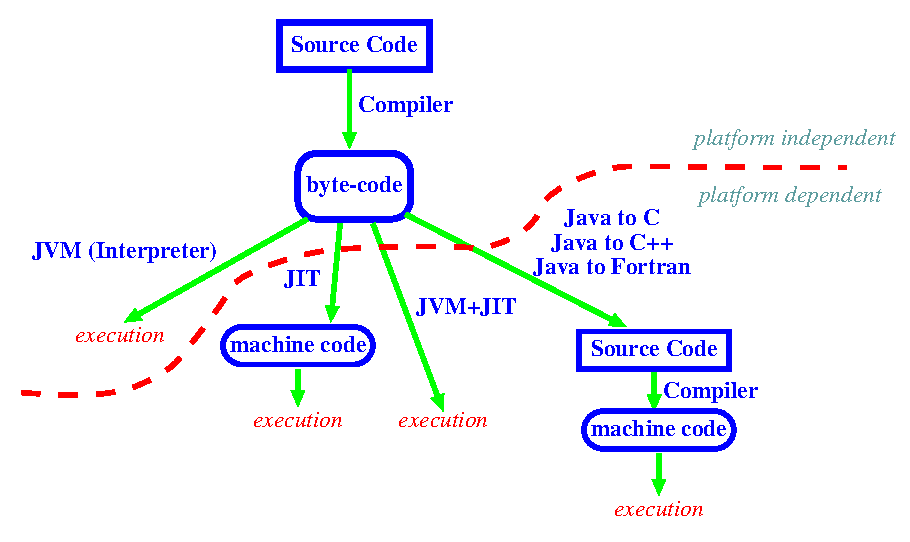
\includegraphics{Figures/Java_Overview.eps}
    \caption{Overview of the Java language execution model.}
    \label{fig:Java_Overview}
  \end{center}
\end{figure}

So for every platform, where a virtual machine is available,
you can execute the byte-code without any compatibility problems.
But the ``look and feel'' can be different, for example Java buttons
in Windows look different from buttons in X11/Motif using a UNIX
operating system. The main reason for the wide availability of Java
is that SUN Microsystems distributes the Java Development Kit (JDK)
freely for a number of important platforms (Windows, Solaris/Linux,
other Unix systems). The JDK consists of a compiler (javac), a
debugger (jdb) and a virtual machine (java)\footnote{Actually there
are some more components like the javadoc command to create HTML
documentation or the jar tool to create zipped packages of
class files belonging together - see later on.}.

The JDK can be downloaded from the internet from the 
\href{http://www.javasoft.com}{JDK Javasoft link page}.
The newest version (as of the time of writing) is 1.1.7. 
There is already a beta version for the JDK
of the new Java 1.2 language specification. Throughout the book,
we will use the Java 1.1 language version and the JDK 1.1.7.

The only additional thing necessary to have a Java programming
environment is an text-editor to write the Java programs. For that
you should use your favorite editor, e.g. emacs or xemacs, which are
also freely available and have nice Java editing modes.

There is also a freely available IDE (Integrated Development 
Environment) called \href{http://www.freebuilder.org/}{FreeBuilder}.
This is a complete environment to write Java programs comfortably,
which is the first under the GNU license. It is still in alpha
development stage, but it already comprises a lot of features. Of
course, there are many commercial ones available, like SUN's Java Workshop.

Opposing to other languages, which use the ASCII character set, Java
uses the Unicode character set \href{http://unicode.org}{(Unicode WWW
Homepage)}. 
Unicode consists of characters represented
by 2 bytes instead of 1 byte like in the ASCII set. So you can not only
use 256 different characters (ASCII) but you can use all the 38885 different
characters available in the Unicode set (Version 2) for writing a Java program.
This means you can name your variables using for example Japanese or Greek
characters. Right from the beginning, Java is an international language.

Java is also case sensitive and doesn't need any special characters
to mark continuation lines. 

Comments are used just like in C and C++.
You can use either the /* \ldots */ syntax (borrowed from C) for
multi-line comments or the // syntax (borrowed from C++) for single
line comments. Additionally you can use /** \ldots */ for comments
to automatically generate a HTML documentation file for the class
defined in the file. We will see later on how this can be achieved.
 
\subsection{The ``HelloWorld'' Program}
\label{sec:HelloWorld}
Now let's start with the traditional ``Hello World'' program written
in Java.

\subsubsection{Application}

\inputlisting{Listings_Java/HelloWorld_Application.java}
You have to save the program in a file called 
\verb|HelloWorld_Application.java|.
To execute the above example you have to type in the commando line the
following:
\begin{itemize}
\item Compiler: \verb/javac HelloWorld_Application.java/  
  $\Longrightarrow$ produces HelloWorld\_Application.class 
  in the same directory.
\item JVM:  \verb/java HelloWorld_Application/
\item Output on screen: \verb<Hello World !<
\end{itemize}
Let us now try to understand the above code. The program consists of
three lines. 

In the first line the program declares 
with the help of the \texttt{class} statement a class called 
\verb|HelloWorld_Application|. 
The identifier following the \texttt{class} statement is
the name by which the class will be referenced. Each Java program
is a class. The curly bracket appearing after the class name
\verb|HelloWorld_Application| introduces the following class member. 


In the second line the \verb|main| method is introduced. The main
method is declared \verb|void| because the method does not return a
value. The main method is executed when you run the class as an
application. In the present case the only parameter, the argument
of the main method, is an array of String object.

In the third line the method \verb|println| of the system class out
is invoked. This method simply prints a string and terminates with a 
new--line  command.

You have just written and executed your first application in
Java. Please, do not worry if you do not understand everything. You are
not expected to understand everything at this stage.


\subsubsection{Applet}
\label{sec:Applet}

Java offers another possibility to execute code, so called Applets.
In contrast to the stand--alone Java application which starts at
\verb!main! and runs until it is completed, the applet is a kind of
sub--program which runs under the control of some other program.
Usually, applets are (small) Java programs, which are started by a 
server program,
e.g. a WWW browser like Netscape Navigator\footnote{You need at least 
version 4.06 or patches for earlier versions to use all features of Java 1.1}, 
the Internet Explorer\footnote{Seems to run Java 1.1 programs since
version 4.}(Don't),
HotJava or the appletviewer\footnote{included with the JDK.}.

The big difference between an applet and an application is that
applets are not allowed to do certain things. For example applets
do not have access to local file systems, so it is not possible
to save data on the file system from an applet. It is also not
possible for an applet to issue a print command, the process of
printing has to be initiated by the server (browser). 
And an applet is not allowed to do time consuming tasks like
long computations. This has to be kept in mind, when writing
applets.


The ``Hello World'' example written as an applet has the following form:
\inputlisting{Listings_Java/HelloWorld_Applet.java}

Applets have to be derived from the applet class
\verb|java.applet.Applet|, which include the principal facilities of
the Abstract Window toolkit (AWT) and the interface with X/Motif on
Unix, Windows on PC, and Mac-OS on Macintosh platforms.
As you can see there is no main method in an applet. Instead if an applet
is started by a server, the init() method is executed first. There is also
a start() (stop()) method, which is executed if the applet becomes
visible (disappears) in the server window (e.g. by scrolling in the
Netscape Navigator window).

Many methods are available to set up the display in an assigned applet area.
The paint() method appearing in the ``Hello World'' applet is
responsible for the visual part of the applet. It uses a canvas
(drawing area) with a size defined by the calling HTML file. In our case
this HTML file could look like:
\inputlisting{Listings_Java/call_HelloWorld_Applet.html}
The code parameter given in the HTML file defines the name of the applet
to be run. Because there is no init() and no start() method in our
example, the paint() method gets executed by the browser (or appletviewer).
The size of the canvas has to be given in pixels explicitly in the
HTML file.

To run the applet you can either type
\begin{itemize}
\item \verb|appletviewer  call_HelloWorld_Applet.html| or
\item use the following URL in the browser: \\
        \verb|PATH_TO_CLASS_AND_HTML_FILE/call_HelloWorld_Applet.html| \\
        e.g. \verb|/home/user/java/call_HelloWorld_Applet.html|
\end{itemize}

The question arising now, when to use an application and when to use
an applet, is difficult to answer. In the following chapters we will 
decide for each program
separately, which way to go. Time consuming calculations should
definitely be written as an application, small programs can be
written as an applet of course.

In Java 1.1 a new package (see later) was introduced, which allows
so called ``trusted applets''. These are specially signed libraries,
which are signed with a key by a person you trust. Only if the
signature is valid and you trust that person, the ``trusted applet''
has access to the local files system -- it basically can do everything
an application could do on your machine. This is already implemented with
the appletviewer, in different ``servers'' it might work or not. In the
future this will be extended to a more extensive set of rules for the
allowed methods of an applet.

A last remark concerns the documentation for the programs. We have
learned, that we can include documentation comments using 
\verb|/** .... */|. These comments are processed by using the
\verb|javadoc| command from the JDK. If you run the javadoc command as: 
\begin{verbatim}
  javadoc HelloWorld_Application.java HelloWorld_Applet.java  
\end{verbatim}
you get some HTML files: packages.html, tree.html, AllNames.html,
HelloWorld\_Applet.html, HelloWorld\_Application.html. All these
files describe the written classes. The tree.html gives a tree
showing the relatives of the class. The package.html gives the
package structure (not used here). The most important file is the
AllNames.html, which is an index of all written programs in this package
(for an introduction to packages see later).

If you load AllNames.html into a browser, you get the HTML file shown
in figure \ref{fig:javadoc1}.
\begin{figure}[htbp]
  \begin{center}
    \leavevmode
 \includegraphics[width=8cm]{Listings_Java/AllNames.eps} 
    \caption{The output of the \texttt{javadoc} command from the JDK.}
    \label{fig:javadoc1}
  \end{center}
\end{figure}
Now you can click on the link HelloWorld\_Applet and you get the
documentation for that class and analogous for the HelloWorld\_Application
class (see figure \ref{fig:javadoc2}).
\begin{figure}[htbp]
  \begin{center}
    \leavevmode
  \includegraphics[width=6cm]{Listings_Java/HelloWorld_Applet.eps}
  \includegraphics[width=6cm]{Listings_Java/HelloWorld_Application.eps}
    \caption{The output of the \texttt{javadoc} command from the JDK.}
    \label{fig:javadoc2}
  \end{center}
\end{figure}
The missing graphics on the right of figure \ref{fig:javadoc2} 
are available in the Java documentation of the
JDK and just has to be copied into a subdirectory called \verb|images| 
of the HTML directory. Then it looks like the figure on the left.

%%%%%%%%%%%%%%%%%%%%%%%%%%%%%%%%%%%%%%%%%%%%%%%%%%%%%%%%
\subsection{Variables}
\label{sec:Variables}

Essentially, Java distinguishes between two types of variables,
primitive data types and reference data types.
\subsubsection{Primitive data types}
\label{sec:primitive_data_types}
We already mentioned that in Java each variable or expression has a
definite type and that each type has identical size and behaviour on
all Java implementations.  Java has built in primitive data types
to support integer, floating--point, boolean, and character values.
The primitive data types of Java for integers, floating--points,
characters and boolean variables are listed in table
\ref{table:primitivedata}.
\begin{table}[htbp]
\label{table:primitivedata}
\begin{center}
\begin{tabular}{l|l|l|l|l}
Type & Contains & Default & Size & Min \\
     &          &         &      & Max \\ \hline \hline
byte  & signed integer & 0 & 8bits & -128  \\
&&& & 127    \\ \hline
short & signed integer & 0 & 16 bit &-32768 \\
&&& & 32767 \\ \hline
int &   signed integer & 0 & 32 bits&-2147483648 \\
&&& &2147483647 \\ \hline
long & signed integer & 0 & 64 bits &-9223372036854775808\\
&&& &9223372036854775807\\ \hline
float & floating--point & 0.0 & 32 bits &$\pm$1.40239846E-45\\
&&& &$\pm$3.40282347E+38\\ \hline
double & floating--point & 0.0 & 64 bits &$\pm$4.94065645841246544E-324\\
&&& &$\pm$1.79769313486231570E+308\\ \hline
boolean & true or false      &  false & 1 bit&\\
&&&       &  \\ \hline
char  & Unicode character & $\backslash$u000 & 16 bits & $\backslash$u000 \\
&&& &$\backslash$uFFFF   \\ \hline
\end{tabular}
\end{center}
\caption{Primitive data types in Java.}
\end{table}


The following comments have to be done. In a Java program every
variable must have a type that precedes its name when the variable is
declared. For example the integer i may be declared as

\begin{verbatim}
int i;
\end{verbatim}


Char values represent characters. They appear in Java between single
quotes, e.g.
\begin{verbatim}
char c = 'C';
\end{verbatim}
A Unicode character is represented by the Unicode escape sequence
$\backslash$uxxxx, where xxxx is a sequence of four hexadecimal digits.


Float and double types have special values that may be the result of
certain floating-point operations. For example in the java.lang.Float
and java.lang.Double classes the special values
\verb|POSITIVE_INFINITY|, \verb|NEGATIVE_INFINITY|, and 
\verb|NaN| (not-a-number) are
defined.

Floating point numbers are expressed as e.g.
\begin{verbatim}
13.       1.3e1        .13E2 
\end{verbatim}
and are considered to be constants of type \verb|double| 
unless they are specified with \verb|f| or \verb|F|, which makes them
then \verb|float| constants.

In Java strings are not a primitive type. Java provides a String
class to deal with sequences of character data. The java string
class provides methods to operate on String objects.

All variables in Java are initialized automatically, as soon as they
are declared. All primitive types get initialized to zero, the boolean type
to false and all objects (remember they are references) are initialized
to \verb|null|. So there is no ambiguity like in other languages, if
a variable has a defined value at certain points of the program. 
Although Java forces you to include sometimes a statement to
initialize variables, just to make easier to read source code.
We will see an example for this later on, when we discuss loops
and calculate averages of sequences of numbers.

\subsubsection{Reference data types}
\label{sec:Reference_data_types}

All non-primitive data types in Java are objects and arrays. They are
called also ``reference types'' because they are handled by
reference. For example you may pass the address of an object, which is
stored in a variable, to a method. In contrast, primitive types are
always passed by value.


%%%%%%%%%%%%%%%%%%%%%%%%%%%%%%%%%%%%%%%%%%%%
\subsection{Casting, Wrapper Classes}

Java uses a clear strategy to convert the primitive data types to 
other primitive ones. In a calculation Java always converts (casts)
the less precise type to a more precise one. So if you multiply an
integer and a float value, it converts automatically the integer to
a float and then multiplies both values. If you want to convert
a value explicitly you can use the cast operators (like in C and C++).
Just write the primitive type in round brackets in front of the value to
be converted, e.g. \verb|result=(double)a*b| casts \verb|a| to 
a double value and
then multiplies it with \verb|b|, assigning the result to \verb|result|.

A common problem is to convert from strings to primitive types and
vice versa. Because strings are objects and not primitive types, we
need a method for the conversion. For that reason Java has so called
wrapper classes in \verb|Java.lang| for all the primitive types. 
These classes provide all the necessary methods for all types of
conversion. The \verb|valueOf()| method always converts a string
to the corresponding wrapper class of a primitive type, e.g. 
\begin{verbatim}
        double a;
        String text;
        a=doubleValue(text.valueOf());
\end{verbatim}
The third line converts the string to the \verb|Double| class and then
the \verb|doubleValue()| method converts to a double primitive type.
For the other types you just have to substitute float or int 
for double.
 
Another method, later used in the \verb|ParamApplet.java| program is
the \verb|Integer.parseInt()| method, which gives back a primitive
type integer instead of the wrapper class like \verb|valueOf()|.
This simplifies the conversion a little bit. For the example, see
\verb|ParamApplet.java| in line 11. But this method is only 
available to Integer, Long and Byte wrapper classes, NOT for
Float and Double. In this case you have to use the \verb|valueOf()| and
\verb|doubleValue()|, \verb|floatValue()| methods.

To convert a double value to a string you have to use the \verb|toString()|
method, which is available for all primitive data types. 



%%%%%%%%%%%%%%%%%%%%%%%%%%%%%%%%%%%%%%%%%%
\subsection{package and import statements}
Because Java was designed to be able to load code distributed
over the whole internet, you have to avoid name conflicts
between the programs (classes). The solution in Java is to put
every class in a \emph{package}. A package  is a group of related
and possibly cooperating classes.

The name of the package is given
at the beginning of a file before the actual program (class)
definition starts. So for example if we put the statement
\begin{quotation}
  \verb/ package de.freiburg.simulation; / 
\end{quotation}
at the beginning of the ``Hello World'' application, we can compile
the application with \verb/javac HelloWorld_Application.java / like before.
But to run the application we have to use
\begin{quotation}
  \verb/ java de.freiburg.simulation.HelloWorld_Application / . 
\end{quotation}
You are wondering why the program does not start? It cannot, because
there is one more thing to know. Java is looking for programs (classes)
in the directory structure given by the class name. So
for the example above you have to put the \verb/HelloWorld_Application.class/ file
in the directory \verb|de/freiburg/simulation/| and issue the command
in the directory, where the directory tree starts.

You could also use an environment variable called \verb|CLASSPATH|. It
describes the directories to search for the class files. So if the
\verb|CLASSPATH|-variable includes \verb|/home/user/java| you can
start the above example in this directory, if the class is in the 
subdirectory  \verb|de/freiburg/simulation/|.

All the standard commands (classes) of Java are stored in a central jar
file, which is additionally packed to save disk space. These classes
are always searched, no matter the \verb|CLASSPATH|-variable is set to.

If you are not using the package command at all, Java uses the empty 
package. This means you can put your programs in the current directory.
This is not recommended for medium to complex programs, but for
test purposes and very small programs this is very convenient.



Before learning more about the syntax of Java, we have to explain another
statement appearing in the part of any Java program before the actual
definition of the class: the \verb|import|-statement. With \verb|import|
you can make classes available, so you don't have to use the fully
qualified name to the class. So if you would like to
use the HelloWorld class from above in your programs, you could either
type \verb|de.freiburg.simulation.HelloWorld()| in your program
or you can use
\begin{verbatim}
import de.freiburg.simulation.*;
....
   HelloWorld();
\end{verbatim}
to import all classes in the \verb|de.freiburg.simulation| class.
You can also use:
\begin{verbatim}
import de.freiburg.simulation.HelloWorld;
....
   HelloWorld();
\end{verbatim}
if you just want to import one special class.

We have already made use of the \verb|import|-statement in the ``Hello World'' 
applet. There we have imported the \verb|java.applet|-class, which
defines applets and their behaviour, and the \verb|java.awt|-class, which
will be explained later.
 
There is one class, which is always imported without any import statement:
the java.lang class. This is the fundamental class of Java and it is
implicitly imported for all Java programs, so you do not have to specify
it. For example the System class is in Java.lang, that is why
we did not have to use an import statement in the ``Hello World''
application.  


%%%%%%%%%%%%%%%%%%%%%%%%%%%%%%%%%%%%%%%%%%
\subsection{Simple arithmetics, Conditional Statements and Loops}
\label{sec:Loops}

\subsubsection{Simple arithmetics}
As we already mentioned Java  supports almost all of the standard
C operators. The arithmetic operators that operate on numerical types
are 
\begin{center}
\begin{tabular}{ll}
$+$ & addition \\
$-$ & subtraction                 \\
$*$ & multiplication \\
$/$ & division \\
\% & remainder
\end{tabular}
\end{center}
The $+$ operator can also be used to concatenate strings, as we will
see later in an example in section \ref{sec:Parameter}.

It is important to remark, that in Java integer division truncates
toward zero (7/2=3, -7/2=-3 and -7/-2=3).

Java has two special operators for increment $++$ and decrement $--$. The 
expression \verb|i++| is equivalent to \verb|i=i+1| except that
\verb|i| is evaluated only once. They can be used as pre- and post-operators,
depending on the position of the symbols, e.g. \verb|i++| or \verb|++i|.
This does not make a difference, if you just have these statements
alone, but in some complex expressions this might make a difference.

Java supports also a standard set of relational and logical operators,
which all yield boolean values. They are listed below

\begin{center}
\begin{tabular}{ll}
$>$  & greater than \\
$>=$ & greater than or equal to \\
$<$  & less then \\
$<=$ & less than or equal to \\
$==$ & equal to \\
$!=$ & not equal to
\end{tabular}
\end{center}


The conditional operators
\begin{center}
\begin{tabular}{ll}
\& \& & conditional AND      \\
$\mid\mid$ & conditional OR
\end{tabular}
\end{center}
operate on  boolean expressions only.

Java has also bitwise operators which operate on integers and on
boolean types
\begin{center}
\begin{tabular}{ll}
\& & and \\
$\mid$ & or \\
$\tilde{}$ & not \\
$<<$ &  shifts bits left filling with zero bits on the right \\
$>>$ & shifts bits right filling with the highest sign bit on the
           left--hand side \\
$ >>>$ & shifts bits right filling with zero bits on the left--hand side 
\end{tabular}
\end{center}

Last not least we have to mention the fundamental assignment operator
$=$. It may be used in combination with other operators, e.g., $+=$
means is incremented by.


\subsubsection{Loops}
\paragraph{for Loops}
For our forthcoming applications the most important control statement
is the \verb|for| statement. It is used to loop over a range of values
from the beginning to the end. Its syntax is
\begin{verbatim}
for (init_expressions; boolean_expr; incr_expressions) {
    statements
}
\end{verbatim}
where \verb|init_expressions| denotes the initial value of the iterated
variable, \verb|incr_expressions| denotes the increment of the iterated
variable. For both you can specify more than one expression separated
by commas ( as in C). This is the only place, where you can use these comma
separated lists.

At the beginning of the \verb|for| loop the boolean expression
\verb|boolean_expr| is evaluated. If its value is found to be 
\verb|true| the statement is executed repeatedly with increment
\verb|incr_expr| until the value of the boolean expression is found to
be \verb|false|.

As an example demonstrating the use of
\verb|for| loops we want to write a program to calculate the mean of
a given number of random numbers. One possible implementation
could look like this:
\inputlisting{Listings_Java/DataMean.java}

Here we used the class \verb|java.util.Random| which allows for
the creation of random numbers. If we don't supply a seed, as is the
case here, it just uses the time to initialize the generator. The
initialization takes place in line 10, where a new generator is created.
You can check this by running the application more than once and comparing
the means -- they should not be the same. 

The \verb|next.Double()| method returns a new random number of type
double (for a float use rand.Float()). You can also create normally 
distributed random numbers with the \verb|Random.nextGaussian()| method.
The remaining parts of the program should be self explaining.


\paragraph{while and do--while}
Java offers also the possibility to use other loop constructs, the
\verb|while| and the \verb|do-while| loop. There syntax is
\begin{verbatim}
while (boolean_expression)
 statement
\end{verbatim}
and
\begin{verbatim}
do
  statement
while (boolean_expression)
\end{verbatim}
It is important to observe that in the first construct the boolean
expression is evaluated \textit{before} the statement is executed, while in
the second construct the boolean expression is evaluated \textit{after} the
statement has been performed!

In order too give an example we write down an equivalent code using
the
\verb|while| statement of the \verb|for| loop of the
\verb|DataMean.java| program. Lines 13 to 15 have to be replaced by
\begin{verbatim}
int i;
while(i<N){
  mean += rand.nextDouble();
  i++;
}
\end{verbatim}

\subsubsection{Conditional Statements}
\paragraph{if-else}
The \verb|if| statement is the fundamental form of conditional control
of flow. It allows to choose, whether the statements that follow it are
executed or not. Its syntax in Java is
\begin{verbatim}
if (boolean_expression) {
   statement1
}
else if (boolean_expression) {
   statement2
}
else {
   statement3
}
\end{verbatim}
First, the boolean expression is executed. If the value is \verb|true|
then \verb|statement1| is performed, otherwise if there is the
optional \verb|else| statement \verb|statement2| is executed. Of
course, \verb|if-else| constructions can be nested, i.e., an
\verb|if-else| conditional control flow, can be placed within another
\verb|if-else| statement.

\paragraph{goto}
We already remarked that Java does not have a \verb|goto| instruction
to transfer control to an arbitrary statement in a method. To handle
with situations where other languages have a \verb|goto| Java provides
the labelled \verb|break| and \verb|continue| statements. Labels are
typically used in blocks and loops and precede statements
\begin{verbatim}
label: statement
\end{verbatim}
The \verb|break| statement is used to exit from a block, e.g. to break
out of a loop. E.g., an unlabeled \verb|break| terminates the innermost
\verb|for|, \verb|while| or \verb|do|.

The \verb|continue| statement is used only within loops. It skips to
the end of the loops body and evaluates the boolean expression that
controls the loop. The \verb|return| statement terminates execution of
a method and returns to the invoker. If a method returns no value you
have to use
\begin{verbatim}
return;
\end{verbatim}
if the method has a return type, the \verb|return| must include an
expression for a returned type.

An dieser stelle sollten einige beispiele kommen!!!!!

\paragraph{switch/case}

Another central flow structure is the \verb|switch| statement. It
evaluates an integer expression whose value is used to find an
appropriate \verb|case| label among those listed inside the following
block. The \verb|switch| statement may be used to replace nested \verb|if-else|
statements that determine what is the output for each number. The
\verb|switch| statement works only if the value being tested is a
primitive integral type and when the value is tested against constant
values. the basic syntax of the \verb|switch| statement is
\begin{verbatim}
switch(expression) {
    statements
}
\end{verbatim}
After evaluating the expression, the switch statement executes
certain code within the block depending on the integral value of the
expression. This information is indicated by the integer label following
the \verb|case:| statement. If there is no \verb|case:| label that
matches the value of the expression, the \verb|swich| command executes
the code following \verb|default:|, if there is one. Otherwise,
\verb|switch| does nothing.

An example of the use of the \verb|switch| statement is found in the
simple program \verb|DiceGame.java| 

\inputlisting{Listings_Java/DiceGame.java}

%%%%%%%%%%%%%%%%%%%%%%%%%%%%%%%%%%%%%%%%%%%
\subsection{Parameters from the command line or from a html file}
\label{sec:Parameter}

The access of parameters given on the command line is as easy as it
is in C and C++. The parameters are stored as strings in Java and
are given as the parameters to the main() method of the application.
That is the reason for the Syntax:
\begin{quotation}
  \verb|public void main(String[] args) |
\end{quotation}
It means that the array \verb|args| (see section \ref{sec:Arrays}
for an explanation of arrays) contains the parameters. Each parameter
is separated with a space in the command line. Here is an example of a 
program using command line parameters:
\inputlisting{Listings_Java/ParamCommandLine.java}
So if you run the program as \verb|java ParamCommandLine 12 34 abcd t5|
the output on the screen will be
\begin{verbatim}
 Parameter No. 0 : 12
 Parameter No. 1 : 34
 Parameter No. 2 : abcd
 Parameter No. 3 : t5
\end{verbatim}
and if you don't supply parameters it will be
\begin{verbatim}
 NO parameters specified !
\end{verbatim}
We also see the concatenation of strings in the output statement.
And because you can only supply one argument to the  \verb|println()|
method, you have to concatenate all outputs to one long string.

A little bit different is the behaviour of applets, because there is
no command line. But there is also a way to transmit parameters from 
the calling HTML file to the Java applet. In the HTML file you can
specify \verb|<PARAM>| attributes like here:
\inputlisting{Listings_Java/ParamApplet.html}

In this case we supply two parameters, called \verb|NumberofPoints| and
\verb|DisplayText| to the Java applet. The value is given in the string
behind the keyword \verb|value|. The Java applet to this HTML file
could look like this:
\inputlisting{Listings_Java/ParamApplet.java}

In the \verb|init()| method we get the parameter \verb|NumberofPoints|
and convert it to an integer using a wrapper method. The string 
of the parameter \verb|DisplayText| doesn't have
to be converted. Then in the \verb|paint()| method we display
the transmitted parameters on the screen. The output in the 
appletviewer or in Netscape should look like this:
\begin{verbatim}
  Parameter NumberofPoints is 10000

  Parameter DisplayText is "This_is_a_test_parameter!"
\end{verbatim}

%%%%%%%%%%%%%%%%%%%%%%%%%%%

\subsection{Arrays}
\label{sec:Arrays}

Before discussing the notion of classes and objects, we want to introduce
another reference type: the array. They are actually objects, but
Java provides many special commands for arrays, which makes them a 
little bit special.

The first question is how to create arrays and how to destroy them.
The destruction is easy to explain: it is done automatically
by the garbage collector (like for all objects). This is different to
other languages like C, C++ and Fortran 90, where you explicitly
have to destroy (free) the allocated memory. 

To create an array you have to use the \verb|new| keyword used for
creating (instantiating) objects. So to create a one dimensional
array with 10 elements you use:
\begin{verbatim}
        int intarray[] = new int[10];
\end{verbatim}
This also sets all the elements to zero. But this is only true for 
primitive types. Arrays of reference types (objects) are created the
same way, but the elements consist of references to the elements. The
elements themselves are NOT initialized and have to be created too.
An example for this is a two dimensional array as we will see soon.

Indices of arrays in Java start with zero as in C and not with 1
as in Fortran. No negative indices are allowed in Java. The length
of an array (meaning the number of elements) is always given
by the \verb|.length| field. For the array above you get the number
of elements by using \verb|intarray.length|. We have already met
this notation when we discussed the command line parameters.

You can also create the array and initialize it right away by using
(also in Java 1.0):
\begin{verbatim}
        int intarray[] = {1, 2, 3, 4, 5, 6, 7, 8, 9, 10};
        int[] intarray = {1, 2, 3, 4, 5, 6, 7, 8, 9, 10};
\end{verbatim}
or one step further, create an array of objects (here strings) and
create the elements in the same step:
\begin{verbatim}
        String stringarray[] = {"a","b","c","d","e","f","g"};
\end{verbatim}
In Java you can even put the brackets behind the type instead of the
variable name (not possible in C). So it does not matter if you
write \verb|int intarray[];| or \verb|int[] intarray;|.

In Java 1.1 you can also use \emph{anonymous arrays}:
\begin{verbatim}
        String[] texts;
        texts = new String[] = {"a","b","c","d","e","f","g"};
        System.out.println(new char[] {'h','e','l','l','o'});
\end{verbatim}
So you can create and initialize arrays without even using a variable.

Multidimensional arrays are also supported. Just like in C they are
arrays of arrays. For example
\begin{verbatim}
        double matrix[][] = new double[10][10]; 
\end{verbatim}
creates a 10 by 10 matrix, meaning that you have created 10 arrays
of type \verb|double[10]|. An important point to make is that you
do not have to specify all dimensions at once. You can for example
create a triangular matrix by submitting:
\begin{verbatim}
        double matrix[][] = new double[10][];
        for (int i=0; i<10; i++) {
                matrix[i] = new double[i+1];
        } 
\end{verbatim}
To access multidimensional arrays you can also use one dimensional
array syntax (as in C). If you have a two dimensional array 
you can access the element [i,j] by accessing the element [i+j*columns]. 

Now let's look at an example using arrays. We have rewritten the program
\verb|DataMean| above to calculate the average of random 
numbers by using arrays.

\inputlisting{Listings_Java/DataMean_Array.java}

Here we first declare a double array called \verb|RandomNumber| and
create it in Line 13. Then we store the random numbers in the array
and afterwards calculate the mean.
The last important point to note is the copying of arrays. 
You can not just write
\begin{verbatim}
        int[] array1 = new int[] = {1,2,3,4,5};
        int[] array2 = new int[10];
        array2 = array1;                // WRONG ! - ERROR ! 
\end{verbatim}
This would only copy the reference of the array1 object to the array2
object, not the values. To copy arrays you have to use the 
\verb|arraycopy()| method of the java.lang.System class. 
So to copy an array in the above example, you have to write:
\begin{verbatim}
        System.arraycopy(array1,0,array2,0,array1.length);
\end{verbatim}
This copies all elements of array1 to array2 staring from element 0. 
The remaining parts 
of array2 is not created!


%%%%%%%%%%%%%%%%%%%%%%%%%%%%%%%%%%%%%%%%%%%%%%%%%%%%%%%%%%%%%%%%%%%%
%%%%%%%%%%%%%%%%%%%%%%%%%%%%%%%%%%%%%%%%%%%%%%%%%%%%%%%%%%%%%%%%%%%%
\section{Object Oriented Programming - Classes}

%%%%%%%%%%%%%%%%%%%%%%%%%%%
\subsection{Classes and Objects}
\label{sec:Classes_and_Objects}

The biggest step you have to take in mastering Java if you are
coming from the Fortran or C community, is to switch to the object
oriented paradigm. Although C++ programmers are used to objects, there
are quite a number of differences to C++ in Java. That is why Java
is closer to C than to C++.

We have already met a lot of object oriented features 
without discussing them in detail. 
\begin{quote}
A class is a collection of data and methods that operate on that data. In
Fortran or C we call the methods procedures or functions. An object
is an instance of the class, meaning it is a thing to work with. The class
defines the data necessary for the object and the functions which can
operate on them.   
\end{quote}
For example you can have a class ``Car'', which describes all the 
eigenschaften of a car, e.g. type, age, weight, etc. Then you have a
``real'' car, let's say a Ford, 10 years old, 1000 kg, etc. So this
is an object of the class ``Car''. A method would be the calculation
of the monthly cost for the car. 

An example already familiar to us, is an array. If you have an array 
object you can call the method \verb|length| to get the number of
elements of the array. 

So what is the difference to the standard function approach here?
Instead of using function arguments you supply the argument by 
putting them in front of the method separated by a point. 
For example to calculate the mean of an array of doubles, you can
either write a method which takes the array as an argument (like you would
in Fortran or C): \verb|mean(array[])| or you can use the object
oriented feature: 
\begin{verbatim}
        Data dat = new Data(); 
        result = dat.mean();
\end{verbatim}
It is up to you, which version you prefer. But because all programs are
actually classes in Java you have to understand at least the 
most fundamental things about object oriented programming. For a detailed
discussion and introduction, see \cite{javanutshell}.

Just to remind you again, strings are objects and not primitive 
types. To use strings you first have to declare and instantiate a string
object. Here are three possible ways of doing it:
\begin{verbatim}
        String text;
        text = "Test String";
        text = new String();
        text = new String("Test String");
\end{verbatim}
The first line only declares a string object called text and does not
allocate (instantiate) the memory for the value of the object, just
the reference to the value.

As an example for the most important issues about objects, we want to
write a class, which calculates random numbers by different methods and
for different distributions. To that end we write a class 
\verb|RandomNumber|. It has three fields (variables), two of them are
defined with the \verb|final| keyword. This is the equivalent to the
const keyword in C. A final field can not be changed anymore.
The \verb|static| modifier defines a field (variable), which is belonging
to the class and not to the object. So every object of that class 
has the same value for a \verb|static| field. The \verb|public| modifier
on the other hand defines a field or method, which is special to 
an object not to the class -- this is also called an instance field or
method, the \verb|static| version is called a class variable or method.
\begin{table}[htbp]
  \begin{center}
    \leavevmode
    \begin{tabular}{l|p{8cm}}
     Modifiers &                                 \\ \hline \hline
     final & variables may not be changed, classes may not be 
                                   subclassed\\\hline
     public & accessible from anywhere\\ \hline
     static & defines a top-level class, a class variable (field) or 
                 a class method\\\hline
     private & only within the defining class visible, not in other 
               packages, even if subclass of this class\\\hline
     protected & accessible within the package in which it is defined and
                 within subclasses\\\hline
     (none) & accessible only in its package\\
    \end{tabular}
    \caption{Overview of some available modifiers in Java. For a complete
      overview take a look at page 230-234 in \cite{javanutshell}.}
    \label{tab:modifiers}
  \end{center}
\end{table}

\inputlisting{Listings_Java/RandomNumber.java}
Class variables and methods are the closest relatives to global 
variables in all the other languages. They are accessible from all
classes, but still are belonging to a class. So you could have two
class methods with the same name, but for different classes.

An important part of any class is the constructor of the class. This is
the method (function), which is called when an object of this
class is instantiated. Here in our example, we just set the seed. As 
you can see you have to supply the seed, when instantiating the
generator. Most of the constructors don't even need a parameter to 
instantiate the object. 

Then the method \verb|nextRand()| is defined and returns the next
random calculated using a congruential method (see later in this
book). The return type of methods always has to be specified, if
there is no return value you have to use the \verb|void| statement
(as in C). The value to be returned is specified by the return keyword.

Now we have to write a program (class), which uses this class to 
calculate the average of some random numbers.
\inputlisting{Listings_Java/UseRandomNumber.java}
The class is called \verb|UseRandomNumber| and just contains the
main method. First we instantiate (create) an object of class
\verb|RandomNumber|. Then we create an array and in a loop we
create \verb|N| random numbers using the \verb|nextRand()| method
of our class applied to the object we just created. The remaining
part has already been explained.

A second example demonstrates how to create a class for calculating
some statistical measures for data sets. 

Listing Moment Calc. (???)

\subsubsection{Extending (Inheritance) and Overloading Classes}
Often you want to define subclasses, which should inherit all
the methods and fields from another class. This is easily done
in Java by extending a given class. 

You can reference the super (parent) class by applying the
\verb|super| modifier in front of a method or variable of
the parent class. And the \verb|this| modifier always refers to
the actual class. 

If you define a class to be final, it can not be extended.
For example the java.lang.System class is a final class.

Different from C++,  you can not inherit from more than one class
in Java, meaning that there is always only one superclass for each
class. 
The only way of having multiple inheritance is by using
interfaces, which we will not cover in our introduction.

If you write a subclass you can overwrite methods already defined
in the super class. This is called overloading of methods,
analogous to the C++ overloading. But in C++ you can even
overload operators like +, -, etc., which is not possible (in Java 1.1) yet.

A simple example is given by the
HelloWorld\_Applet.java program in section \ref{sec:Applet}.
There we have extended the Applet class of the Java.applet package
and therefore making our program a subclass of the Applet class.
So we inherited all the methods and fields of that class. Then we
overloaded the \verb|paint()| method to display our message. 
In the words of object oriented programming, writing an applet is
called: defining a subclass of the Applet class and overloading
the methods of the Applet class as necessary.

\subsubsection{Overview of all packages in Java 1.1}

Here we list all the standard packages included in the Java 1.1
language standard. The important packages (in our point of view)
are written in small caps.
\begin{description}
\item[\textsc{java.applet}] includes the superclass of all Java applets (small package)
\item[\textsc{java.awt}] the Abstract Windowing Toolkit (large package)
\item[java.awt.datatransfer] provides data exchange between programs
\item[\textsc{java.awt.event}] event handling for the AWT (Mouse, etc.)
\item[java.awt.image] rarely used classes for image processing (use AWT) 
\item[java.awt.peer] rarely used interfaces for the AWT
\item[java.beans] interfaces and classes for beans programmer
\item[\textsc{java.io}] all the input/output classes (very big)
\item[\textsc{java.lang}]  central Java language classes (largest package)
\item[java.lang.reflect] part of the Java Reflection API (small)
\item[\textsc{java.math}] arbitrary precision arithmetic (small)
\item[java.net] networking package
\item[java.text] for writing internationalized programs (date, time, etc.)
\item[\textsc{java.util}] useful classes, often used, e.g. millisecond time,
  calendar, random numbers, vectors, etc.
\item[java.util.zip] data compression and decompression classes
\end{description}

%%%%%%%%%%%%%%%%%%%%%%%%%%%%%%%%%%%%%%%
\subsection{The System class: Screen-Output and Keyboard-Input}

Now we are in a place to discuss the \verb|System.out.println()| statement
already used in the ``HelloWorld'' program. This is calling the
\verb|println()| method of the \verb|PrintStream| class of the java.io 
package. And the \verb|out| is a variable from the System 
class of the java.lang package, referencing the \verb|PrintStream| class. 

There are also two more variables called \verb|err| and
\verb|in| for error output and data input. 
The java.lang.System class in general provides an platform-independent 
interface to some system functions.

Here an example, which demonstrates a few things already learned and
explains how to get input from the keyboard:
\inputlisting{Listings_Java/System_Class.java}
It waits for an user input and just echoes the typed characters
until you type the word ``Java''. Let us analyze the program:

First look at line 19, where we have used the \verb|print()| method
of the System class. It does the same as \verb|println()|, but does not
jump to the next line after the output.

Then take a look at line 23, where we compare two strings. As you see
you have to use the \verb|equals()| method of the String class to
compare the value of two strings and not the references. 
In line 25 we use the string concatenation operator $+$ for the output.

The actual input takes place in line 21, where we assign the input
to the string \verb|line|. The method used is \verb|readLine()|, which
is a method of the \verb|BufferedReader| class. It reads input until
a carriage return is reached. The actual object of the 
\verb|BufferedReader| class is created in line 13. To that end we have
to create a Reader class for the \verb|InputStream| called \verb|in|
just mentioned above (this is done in line 11).

Because we are using I/O commands, we have to take care of exceptions
which can occur during the I/O. For that reason we have to use the
\verb|throws IOException| statement in the definition of the main
class (see line 7).

A last remark concerns the escape codes used in line 15 and line 25.
The first one displays a quotation mark and the second one is just a 
newline character. These are analogous to the C escape codes.

Although this looks very complicated, if you don't want to go into
details, just copy this part to your own program and your are done.
But after you got used to object oriented programming you won't have
any problems understanding the code above anymore.


\subsection{Standard Mathematical Functions and Mathematical Libraries}
\label{sec:Standard_Math}

The standard mathematical functions of Java are declared in the 
Java.lang.Math class and contains sine, cosine, logarithm, exponential,
square root and much more. Do not confuse this class with the
java.Math class, which was introduced to Java 1.1 for arbitrary
precision arithmetic -- we are not discussing this.
Here is a table of the methods:
\begin{table}[htbp]
  \begin{center}
    \leavevmode
    \begin{tabular}{ll}
      abs() & absolute value \\
      acos()/asin()/atan() & arcus cosine/sine/tangent \\
      sin()/cos()/tan() & sine/cosine/tangent\\
      exp() / log() & exponential and natural logarithm \\
      ceil()/floor()/round()/rint()&rounding of values (see test program)\\
      pow() & power\\
      min( , ) / max( , ) & minimum or maximum of two values \\
      sqrt() & square root of a double \\
      random() & random numbers (use java.util.Random class)\\
      IEEEremainder() & special remainder function \\
    \end{tabular}
    \caption{Overview of the mathematical methods available in Java 1.1 in the java.lang.Math class.}
    \label{tab:math_table}
  \end{center}
\end{table}

These are all class methods, so they can be called from anywhere.
Here are some examples:
\begin{verbatim}
 a=Math.exp(2.1);        // e to the 2.1
 distance = Math.sqrt(Math.pow(x,2)+pow(y,2));  // Euclidean dist.
\end{verbatim} 
By the way, there is no easy import statement to avoid the Math in front
of the methods, you always should use it, although it seems 
tedious.

Here is a test program for the three rounding methods available:
\inputlisting{Listings_Java/Test_Roundings.java}
And the output is:
\input{Listings_Java/Test_Roundings.output}


Unfortunately these easy and important methods are not part of the
standard Java language. But Visual Numerics, a software company,
has proposed a standard class for statistical functions, which are
essential for all statistical problems. They also supplied a new class
for complex numbers. This library is called the Java Numerical Library
(JNL) and is free. 

There are also other classes, which extend the standard Java language
for matrix computations (BLAS) and much more (e.g. the JNT). If we need
them in the course of the book, we will introduce you to them there.


\subsubsection{Summary and Overview}
General structure of a program:
1) package
2) import
3) Classes
4) Interfaces

%%%%%%%%%%%%%%%%%%%%%%%%%%%%%%%%%%%%%%%%%%%%%%%%%%%%%%%%%%%%%%%%%
\section{More Advanced Features}

\subsection{Input/Output}
\label{sec:Input/Output}
Exception Handling, Gnuplot

\subsection{Graphics and Visualization}
\label{sec:Graphics_and_Visualization}
AWT, Graphics

Example: Random Points

Plotting using: Graph2D, Scivis,


\subsection{More Features}
\label{sec:features}
Beans, EPS Output,

\subsection{Online References}
\label{sec:Online_Refernces}


%%%%%%%%%%%%%%%%%%%%%%%%%%%%%%%%%%%%%%%%%%%%%%%%%%%%%%%%%%%%%%%%%
\section{Exercises}
Pi Calculation:
\inputlisting{Listings_Java/Pi_Calc.java}


radioactive decay, e calc.
Moment calulation

%%%%%%%%%%%%%%%%%%%%%%%%%%%%%%%

\nocite{FLANAGAN-EXAMPLES}
\nocite{GOSLING}

%%%%%%%%%%%%%%%%%%%%%%%%%%%%%%%

\bibliographystyle{peter}
\bibliography{V_98,simulit}

\selectlisting{matlab}

